\chapter{Relativistische mechanica}

\section{Botsingen}
We gaan nu terug naar de Speciale Relativiteitstheorie. We zullen allereerst een tweetal botsingen
analyseren, waarbij we gebruik maken van de Lorentztransformaties. We zullen zien dat, indien we
de behoudswetten willen handhaven samen met de Lorentztransformaties, we de definities van impuls 
moeten aanpassen.
\subsection{Elastische verstrooiing}
We nemen allereerst aan dat de
botsing `perfect' is, dat wil zeggen dat geen energie verloren gaat
in verwarming van de deeltjes en wrijving kan worden  verwaarloosd. Denk
hierbij aan twee biljartballen op een perfect gladde biljarttafel. We
noemen dit `elastische botsingen'. We nemen twee deeltjes die met
snelheid $\vec{u}_1$ en $\vec{u}_2$ op elkaar afkomen en na de botsing
een snelheid $\vec{v}_1$ en $\vec{v}_2$ hebben. We schrijven het
behoud van impuls op als:
\begin{equation}
\alpha_1\vec{u}_1 +\alpha_2 \vec{u}_2 = \alpha_3 \vec{v}_1 +\alpha_4 \vec{v}_2
\end{equation} 
waarbij in de Klassieke Mechanica we natuurlijk identificeren:
\begin{eqnarray} 
\alpha_1 & = & \alpha_3 \;\;\;\;\mbox{massa van deeltje 1} \\ 
\alpha_2 & = & \alpha_4 \;\;\;\;\mbox{massa van deeltje 2} 
\end{eqnarray}
oftewel
\[
m_A\vec{u}_1 + m_B \vec{u}_2 = m_A\vec{v}_1' + m_B \vec{v}_2'  
\]
De massa $m$ noemen we de `trage massa' van de deeltjes. In Figuur~\ref{f:bots} is deze botsing weergegeven. 
\begin{figure}[ht] 
\centering
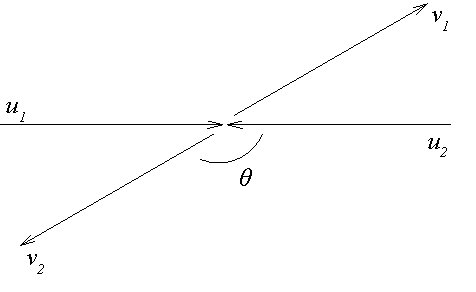
\epsfig{file=u1u2Horiz.pdf, width=0.4\textwidth}
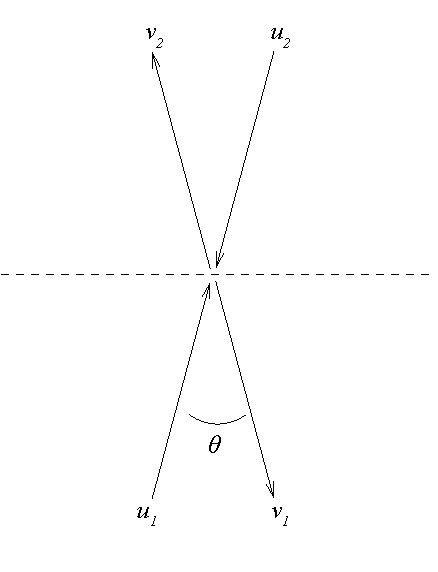
\epsfig{file=u1u2Vert.pdf, width=0.2\textwidth}
\caption{{\sl Elastische botsing tussen twee identieke deeltjes die met gelijke snelheid op elkaar worden afgeschoten. In het rechterfiguur is de botsing `gedraaid' zodat deeltje 1 van onderaf komt en deeltje 2 van bovenaf.\label{f:bots}}}
\end{figure}
In de relativiteitstheorie zullen we een extra snelheidsafhankelijke
term toevoegen in de definitie van impuls. 

De elastische botsingen tussen twee identieke deeltjes die met
dezelfde grootte van snelheid $|\vec{u}|$ op elkaar af worden
geschoten heeft
$|\vec{u}_1|=|\vec{u}_2|=|\vec{v}_1|=|\vec{v}_2|$. Bij deze botsing
wordt wel de richting van de deeltjes veranderd, en de inkomende en
uitgaande deeltjes maken een hoek $\theta$.


We gaan nu deze botsing beschouwen vanuit een co\"ordinatenstelsel dat
meebeweegt met deeltje 1. In dit stelsel heeft deeltje 1 geen snelheid in de
$x$-richting, maar alleen een snelheid in de $y$-richting. We noemen dit snelheid $w$.
Deeltje 2
maakt een hoek $\alpha$ met de $x$-as. Deze situatie is getekend in Figuur~\ref{f:bots2}.
We hebben nu de situatie dat:
\begin{itemize}
\item Deeltje 1 gaat nu `recht omhoog' met snelheid $w_1$ en terug met 
snelheid $w_2$. Deze snelheden zijn aan elkaar gelijk maar tegengesteld. 
\item Deeltje 2 heeft in dit stelsel een grotere snelheid
$\vec{V}$. De $x$-component van de snelheid is $u$ en de $y$-component noteren we als $v$.
\end{itemize}
\begin{figure}[ht] 
\centering
%\includegraphics[width=.35\textwidth]{syllabus.pictures/w1w2onder}
%\includegraphics[width=.35\textwidth]{syllabus.pictures/w1w2boven}
\epsfig{file=w1w2onder.pdf, width=0.35\textwidth}
\epsfig{file=w1w2boven.pdf, width=0.35\textwidth}
\caption{{\sl Links: Botsing tussen twee identieke deeltjes in het stelsel dat meebeweegt met deeltje 1.
Rechts: Botsing tussen twee identieke deeltjes in het stelsel dat meebeweegt met deeltje 2.
\label{f:bots2}}}
\end{figure}


We vragen ons nu af of we een relatie tussen de $y$-componenten van de
impuls van deeltje 1 en 2 kunnen vinden, dus een relatie tussen $w$ en
$v$. Kijk hiervoor naar een ander stelsel $S'$ dat met deeltje 2
meebeweegt. In $S'$ heeft deeltje 2 dus geen $x$-component van de
snelheid, maar deeltje 1 wel. Uit symmetrie-overwegingen volgt dat de
situatie nu precies gelijk is aan die in stelsel $S$, met deeltjes 1
en 2 omgewisseld. Maar voor de transformatie van de snelheden in de
$y$-richting hadden we uitdrukking~\ref{e:vy}, oftewel
\begin{equation}
V_y = \frac{V_y'}{\gamma}\frac{1}{1-\frac{\beta}{c}V'_x}
\end{equation}
 Verder volgt
\begin{eqnarray}
V'_y & = & w \\
V'_x & = & 0
\end{eqnarray}
met andere woorden: we hebben gevonden dat $v=w/\gamma$ (let op, $w$
is de $y$-component van de snelheid van deeltje 1 in $S$, en van
deeltje 2 in $S'$; $v$ is de $y$-component van deeltje 2 in $S$ en deeltje 1 in $S'$).
Merk nu op dat:
\begin{enumerate}
\item De totale snelheid van bewegend deeltje 1 in $S$ en van bewegend deeltje 2 in $S'$ is hetzelfde, namelijk: $V=\sqrt{v^2+u^2}$.
\item Impulsbehoud in de $y$-richting geeft nu
\begin{equation}
\alpha(w) w - \alpha(V) v = -\alpha(w) w + \alpha(V) v
\end{equation}
en let hierbij goed op het verschil tussen $V$ en $v$ en de tekens! We hebben nu
\begin{equation}
\frac{\alpha(V)}{\alpha(w)} = \frac{w}{v} = \frac{w}{w/\gamma} = \gamma \label{e:imprat}
\end{equation}
\end{enumerate}
Neem nu de snelheid $w$ heel klein. In deze limiet is
$\lim_{w\rightarrow 0} v = 0$ en $\lim_{w\rightarrow 0} V = u$. In dat
geval kunnen we de relativistische effecten verwaarlozen en moeten we
de Klassieke uitdrukking voor impuls terugvinden. Dit houdt in dat 
\begin{equation}
\lim_{w\rightarrow 0} \alpha(w) = m 
\end{equation}
en hiermee (invullen in~\ref{e:imprat}) vinden we
\begin{equation}
\lim_{w\rightarrow 0} \alpha(V) = \gamma m = \frac{m}{\sqrt{1-\frac{u^2}{c^2}}}
\end{equation}
We moeten dus de definitie van impuls aanpassen om te zorgen dat deze behouden blijft. Deze relativistische
uitbreiding van impuls is
\begin{equation}\label{e:impuls}
\vec{p} = \gamma m \vec{v}
\end{equation}
Met deze definitie kunnen we de elastische botsingen relativistisch beschrijven. De factor $\gamma$ 
is toegevoegd als gevolg van de transformatie van de snelheid in de $y$ richting.
\subsection{Inelastische verstrooiing}
We zullen nu een heel ander type botsingen beschouwen, namelijk de inelastische botsing. Hierbij 
botsen twee deeltjes op elkaar zonder dat ze terugstoten. Denk nu aan twee klompen klei die
op elkaar worden geschoten en na de botsing een grote klomp vormen. 

\begin{figure}[ht] 
\centering
%\includegraphics[width=.9\textwidth]{syllabus.pictures/2mtotM}
\epsfig{file=2mtotM.pdf, width=0.9\textwidth}
\caption{{\sl Links: Inelastische botsing tussen twee identieke deeltjes. Links in het stelsel waarin
deeltje $M$ in rust is, rechts in het stelsel waarin $M$ een kleine snelheid $\vec{u}$ heeft. 
\label{f:bots3}}}
\end{figure}


Neem twee identieke deeltjes met massa $m$ die een inelastische botsing maken. Beide komen met snelheid $w$ naar elkaar toe. Na de botsing is er \'e\'en stilstaand deeltje over met massa $M$. Klassiek verwachten
we dat geldt $M=2m$.

We beschouwen nu dezelfde botsing vanuit een stelsel dat met een kleine snelheid $u$ in de $y$-richting beweegt. De impuls voor en na de botsing in de $y$ richting levert:
\begin{eqnarray}
\mbox{voor} & p = & 2 \gamma m u \\
\mbox{na}   & p = & M u 
\end{eqnarray}
waarbij we de relativistische definitie van de impuls hebben gebruikt, zie vergelijking~\ref{e:impuls}. We nemen weer de limiet $u\rightarrow 0$ en factor $\gamma$ staat dan voor $\gamma = 1/\sqrt{1-w^2/c^2}$.
We hebben nu dus gevonden dat geldt:
\begin{equation}
M = 2\gamma m = \frac{2m}{\sqrt{1-\frac{w^2}{c^2}}}
\end{equation}
en dus is de massa $M$ na de botsing {\it groter} dan de som van de
twee (rust-) massa's voor de botsing!  Dit is ook het gevolg van de
wet van behoud van impuls. We zullen zien dat de toename van massa na
de botsing afkomstig is van de kinetische energie v\`o\`or de botsing.
\section{Relativistische energie}
We geven eerst het gedachtenexperiment van Einstein waarin de
gelijkheid van energie en massa werd gepostuleerd.  Dit
gedachtenexperiment is ook gepubliceerd in 1905, en is te vinden in de
reader bij dit college. Vervolgens zullen we de energie van een bewegend voorwerp 
beschouwen. 
\subsection{De doos van Einstein}
Als er \'e\'en natuurkundige wet is die iedereen kent, is dat wel de beroemde wet van equivalentie 
tussen massa en energie
\begin{equation}
E= m c^2
\end{equation}
Einstein toonde deze wet eerst aan met een eenvoudig
gedachtenexperiment. In 1905 had hij eerst een verklaring voor het
foto-elektrisch effect gegeven. Dit beschrijft het fenomeen waarbij
licht op een plaatje valt en elektronen losmaakt. De energie van de
elektronen bleek af te hangen van de `kleur' van het licht, en niet
van de intensiteit van de lichtbron. De verklaring werd door Einstein
gegeven door licht voor te stellen als deeltjes, fotonen, elk met een
energie $E_{\gamma} = h \nu$. De constante $h$ is de constante van
Planck en heeft de waarde $h=6,626\cdot 10^{-34} $kg m$^2$ s$^{-1}$, en
$\nu$ staat voor de frequentie van het licht. De impuls van een foton
is omgekeerd evenredig met de golflengte $\lambda$ en wordt gegeven
door $p_{\gamma}=h/\lambda$. Met de uitdrukking $\lambda \nu = c$ is
hiermee gegeven dat
\[
E_{\gamma} = c p_{\gamma}
\]

Het gedachtenexperiment van Einstein (`Einsteins doos') gaat nu als
volgt. Stel je een doos voor, volledig afgesloten van de
buitenwereld. De doos heeft een massa $M$. Aan de linkerkant van de
doos wordt nu een foton uitgestraald door de wand, en vertrekt naar de
rechterkant van de doos. Op het moment van vertrek krijgt de doos een
terugstoot van het vertrekkend foton. De impuls van het foton
wordt gegeven door $p_{\gamma}=E/c$ en de impuls van de terugstoot
door $p=Mv$. Met andere woorden, de snelheid van de doos, $v$, door de terugstoot is gelijk aan
$v=-p/M = -E/ cM$. We hebben hier de klassieke benadering voor de impuls genomen, vanwege de geringe snelheid die de doos oppikt.


Op het moment dat het foton aan de andere kant aankomt, wordt de
terugstoot tenietgedaan en staat de doos weer stil. De doos is dan
verplaatst over een afstand $\Delta x$. Deze afstand is gelijk aan $\Delta x=v \Delta t$,
waarbij $\Delta t$ de tijd voorstelt die het foton er over doet om door de
doos te vliegen, $\Delta t = L/c$ met $L$ de grootte van de doos.
Hiermee is dus de afgelegde afstand $\Delta x=-vL/c = -EL/c^2 M$. 

\begin{figure}[ht] 
\centering
% \includegraphics[width=.5\textwidth]{syllabus.pictures/EinsteinBox}
\epsfig{file=EinsteinBox.pdf, width=0.5\textwidth}
\caption{{\sl De `doos van Einstein'. Voor de uitleg zie tekst.
\label{f:bots4}}}
\end{figure}


Het foton heeft pure energie getransporteerd; geen massa! Maar het
zwaartepunt van de doos, dat geen contact met de buitenwereld heeft, kan door deze
actie van het foton niet verplaatst zijn. Als er een massa $m$ verplaatst zou zijn geweest, 
over de lengte $L$ van de doos, zegt het behoud van het zwaartepunt:
\[
mL + M\Delta x = 0
\]
Nu kunnen we invullen voor $\Delta x$ en krijgen:
\[
 mL - M\frac{EL}{c^2M} = 0\;\;\;\; \mbox{oftewel:} \;\;\;\; L\left(m-\frac{E}{c^2}\right) = 0
\]
en hiermee $E=mc^2$!

Met andere woorden: de pure energie $E$ van het foton is equivalent aan een massa $m$ waarvoor geldt
$m=E/c^2$. Het is aan Einstein te danken dat hij deze relatie algemeen heeft opgevat: energie is 
equivalent aan massa.

\subsection{Energie van een bewegend voorwerp}
Met het gedachtenexperiment heeft Einstein aangetoond dat energie en
massa aan elkaar gelijk zijn via de relatie $E=mc^2$. Voor een
voorwerp dat met een snelheid beweegt, hebben we aangetoond dat de
impuls wordt aangepast, en de relativistische beschrijving wordt
gegeven door
\begin{equation}\label{e:impulsmov}
\vec{p} = \gamma m \vec{v}
\end{equation} 
Zo kunnen we ook postuleren dat de energie van het voorwerp gelijk is aan
\begin{equation}\label{e:energymov}
E = \gamma m c^2
\end{equation}
en we zullen aantonen dat we met deze uitdrukking de juiste Klassieke Limiet verkregen wordt. 
Immers, we kunnen voor lage snelheden benaderen dat
\[
\gamma  = \frac{1}{\sqrt{1-\frac{v^2}{c^2}}} \sim \left( 1 + \frac{v^2}{2c^2} - 
\frac{3}{8}\frac{v^4}{c^4}\right)  
\]
en vinden dus dat
\[
E = \gamma m c^2 \approx mc^2 + \frac{1}{2} m v^2 - \frac{3}{8} m v^4 / c^2
\]
In de limiet voor lage snelheden is dit is precies de kinematische energie $\frac{1}{2}mv^2$ 
plus een constante, $mc^2$. Energiebehoud wordt door dergelijke 
constanten uiteraard netjes intact gelaten.

We zullen nu ook laten zien dat deze definitie voor de energie,
vergelijking~\ref{e:energymov}, overeenstemt met de klassieke relatie
tussen energie en kracht, zoals gegeven in
vergelijkingen~\ref{eq:vermogen1} en~\ref{eq:vermogen2}. We hebben gezien dat verandering van energie
$dE/dt$ teweeg wordt gebracht door het vermogen $\vec{F}\cdot \vec{v}$. Invullen levert:
\begin{equation}
\frac{dE}{dt} = \frac{d\gamma m c^2 }{dt} = \vec{v}\cdot \vec{F} = \vec{v} \cdot \frac{d\vec{p}}{dt}  = \vec{v}\frac{d\gamma m\vec{v}}{dt}
\end{equation}
We zullen nu laten zien dat deze vergelijking inderdaad consistent is. Daartoe vermenigvuldigen we met $2\gamma m$ om tot totale afgeleiden te komen:
\begin{eqnarray}
2\gamma m c^2 \frac{d\gamma m}{dt} = 2\gamma m \vec{v} \cdot \frac{d\gamma m \vec{v}}{dt} \\
c^2 \frac{d}{dt} \left( \gamma m\right)^2 = \frac{d}{dt}\left( \gamma m v\right)^2
\end{eqnarray}
Hieruit volgt dat moet gelden:
\[
c^2 \gamma^2 m^2 = \gamma^2 m^2 v^2 +C
\]
waarbij $C$ een integratieconstante is, en het inproduct $\vec{v}\cdot \vec{v}$ geschreven wordt als $v^2$. Om de integratieconstante te bepalen vullen we snelheid $v=0$ in. Dan is $\gamma=1$ en volgt:
\[
c^2 m^2 = C
\]
zodat we kunnen schrijven
\[
c^2\gamma^2 m^2 - \gamma^2 m^2 v^2 = c^2 m^2
\]
waaruit we kunnen afleiden dan moet gelden dat 
\[
\gamma^2 = \frac{c^2}{c^2-v^2} = \frac{1}{1-\frac{v^2}{c^2}}
\]
hetgeen precies is wat we verwachten voor $\gamma$. Met andere woorden: de relativistische 
uitdrukking voor de energie stemt overeen met de relaties tussen energie en kracht zoals gegeven door de Klassieke Mechanica.




\section{Energie-impuls vector}
We kunnen de relativistische uitdrukkingen voor energie en impuls ook
op een ander manier benaderen. Daartoe keren we terug naar de
vier-vectoren $x=(ct,x,y,z)$, en vragen ons af of er nog andere
vier-vectoren te defini\"eren zijn.

Daartoe laten we ons inspireren door de definitie van impuls in de Klassieke Mechanica: 
\[
\vec{p} = m\vec{v} = \lim_{\Delta t \rightarrow 0} m\frac{\Delta \vec{x}}{\Delta t}
\]
waarbij $\Delta x$ de verplaatsing in de $x$-richting is en $\Delta t$
de tijdsduur. We vragen ons af of hier een equivalente vier-vector van
te maken is in de vier-dimensionale ruimte-tijd. Dit is inderdaad
mogelijk door $\Delta \vec{x}$ te vervangen door de viervector $\Delta x$.
We kunnen echter niet $\Delta t$ in de noemer laten staan, omdat deze niet invariant onder de Lorentztransformaties is. We kunnen wel $\Delta t$ vervangen door het verloop van de eigentijd, $\Delta \tau$,
omdat $\tau$ immers een scalar is. Als vier-vector kunnen we dus schrijven:
\begin{equation}
p =(p_0,p_1,p_2,p_3) =  \left( m\frac{c\Delta t}{\Delta \tau}, m \frac{\Delta x}{\Delta \tau}
, m \frac{\Delta y}{\Delta \tau}, m \frac{\Delta z}{\Delta \tau}\right)
\end{equation}
en de vier-vector $p$ van  een voorwerp heeft nu de richting langs de wereldlijn van dit
voorwerp in de ruimte-tijd. Voor de limiet $\Delta \tau\rightarrow 0$ kunnen we de componenten
van de vier-vector identificeren als:
\begin{eqnarray}
p_0 & = & \frac{E}{c} \\
p_1 & = & p_x \\
p_2 & = & p_y \\
p_3 & = & p_z 
\end{eqnarray}
immers, voor de componenten geldt:
\begin{eqnarray}
\frac{E}{c} & = & m c \frac{dt}{d\tau} = \gamma m c\\
p_x & = & m \frac{dx}{d\tau} = \gamma mv_x \\
p_y & = & m \frac{dy}{d\tau} = \gamma mv_y \\
p_z & = & m \frac{dz}{d\tau} = \gamma mv_z 
\end{eqnarray}
Alle vier deze componenten zijn behouden bij een interactie (d.w.z.
botsing). De componenten zijn niet hetzelfde in elk stelsel $S$ of
$S'$. Wel is de lengte van de vier-vector invariant, met andere
woorden, de uitdrukking
\begin{equation}
\left(\frac{E}{c}\right)^2 - |\vec{p}|^2 
\end{equation}
is hetzelfde in elk stelsel. Deze uitdrukking is gelijk aan:
\begin{eqnarray}\nonumber
|p|^2 & = &  \left(\frac{E}{c}\right)^2 - |\vec{p}|^2  \\
      & = & m^2c^2 \frac{dt^2}{d\tau^2}-m^2\frac{dx^2}{d\tau^2}-m^2\frac{dy^2}{d\tau^2}-m^2\frac{dz^2}{d\tau^2}\\ \nonumber
      & = & m^2\frac{\left(d c^2 t^2 - dx^2 - dy^2 - dz^2\right)}{d\tau^2} \\ \nonumber
      & = & m^2 c^2 \frac{d\tau^2}{d\tau^2} \\ \nonumber
      & = & m^2 c^2
\end{eqnarray}
we kunnen dit schrijven als
\begin{equation}
E^2 - c^2 |\vec{p}|^2 = m^2 c^4
\end{equation}
en dit is de relativistische relatie tussen energie en impuls. Het is
niets anders dan de lengte van de vier-vector $p$. Het `min'-teken is
deze uitdrukking is hetzelfde `min'-teken als we al eerder zagen in de
Minkowski-ruimte: dit maakte de ruimte-tijd fundamenteel anders dan de
Euclidische ruimte.

Merk verder op dat $m$ een invariante grootheid is, die hetzelfde is in alle stelsels. De uitdrukking is
overigens {\it kwadratisch} voor de energie, dus heeft de energie zelf twee oplossingen, namelijk $E=\pm 
\sqrt{m^2 c^4 + c^2 |\vec{p}|^2}$. Dit zal uiteindelijk, wanneer de speciale relativiteitstheorie gecombineerd wordt met de quantummechanica, aanleiding geven tot het bestaan van anti-materie.

De Lorentztransformatie voor de componenten van de vier-vector $p$ kunnen verkregen worden door de componenten in te vullen. Het levert op voor een boost langs de $x$-as:
\begin{eqnarray}
\frac{E'}{c} &=& \gamma\left(\frac{E}{c} - \beta p_x \right) \\
p_x' & = & \gamma\left( p_x - \beta \frac{E}{c}\right) \\
p_y' & = & p_y \\
p_z' & = & p_z
\end{eqnarray}


\subsection{Massaloze deeltjes}
We zien dat de relativiteitstheorie massaloze deeltjes toelaat:
\begin{displaymath}
E = pc
\end{displaymath}
leidt tot
\begin{displaymath}
M = 0
\end{displaymath}
Aangezien uit formules \ref{e:impulsmov} en \ref{e:energymov} volgt dat
\begin{displaymath}
p = \frac{E}{c} \beta 
\end{displaymath}
(ga na) geldt voor massaloze deeltjes dus:
\begin{displaymath}
p = \frac{pc}{c} \beta = p \beta
\end{displaymath}
Hieruit volgt dat $\beta = 1$, dus $v = c$.
M.a.w. massaloze deeltjes bewegen met de lichtsnelheid; zij kunnen niet stilstaan. Het foton
is het bekendste voorbeeld. 

\section{Samenvatting}
De relativistische relatie tussen energie, impuls en snelheid kan worden samengevat als:
\begin{eqnarray}
E\leftrightarrow \vec{p} & \mbox{:} & E^2 - c^2 |\vec{p}|^2 = m^2 c^4 \\ \nonumber
E\leftrightarrow \vec{v} & \mbox{:} & E = \gamma m c^2 \\ \nonumber
\vec{p} \leftrightarrow \vec{v} & \mbox{:} & \vec{p} = \gamma m \vec{v} 
\end{eqnarray}
De relatie tussen de energie, impuls en snelheid wordt gegeven door:
\begin{equation}
\frac{c\vec{p}}{E} = \frac{\gamma m \vec{v} c}{\gamma m c^2} = \frac{\vec{v}}{c} = \vec{\beta}
\end{equation}
dus 
\begin{equation}
\vec{\beta} = \frac{\vec{v}}{c} = \frac{c\vec{p}}{E}
\end{equation}

\section{Enige opmerkingen n.a.v. botsingen} 

In de beschrijving van een botsing tussen een willekeurig aantal
deeltjes kunnen we nog het volgende opmerken. Bij de botsing
zijn de {\it ingaande} deeltjes te onderscheiden van de {\it
uitgaande} deeltjes. Voor een systeem van $n$ ingaande deeltjes en
$m$ uitgaande deeltjes gelden de volgende behoudswetten:
\begin{eqnarray}
\sum_{deeltjes}^n p_x^{in} & = & \sum_{deeltjes}^m p_x^{uit} \\ \nonumber
\sum_{deeltjes}^n p_y^{in} & = & \sum_{deeltjes}^m p_y^{uit} \\ \nonumber
\sum_{deeltjes}^n p_z^{in} & = & \sum_{deeltjes}^m p_z^{uit} \\ \nonumber
\sum_{deeltjes}^n E^{in} & = & \sum_{deeltjes}^m E^{uit}
\end{eqnarray}
Dit zijn de behoudswetten van de botsing: dat wil zeggen dat deze grootheden, impuls en energie, 
voor en na de botsing hetzelfde zijn. Deze grootheden hangen af van het stelsel $S$ waarin we de botsing 
beschouwen. De invariant $E^2-c^2|\vec{p}|^2$ is hetzelfde in elk co\"ordinatenstelsel $S$. Deze grootheid is ook behouden voor het hele systeem, maar niet voor elk deeltje afzonderlijk.

De `massa van een systeem' leidt soms tot verwarring. Een lichaam met grote temperatuur heeft meer energie en 
dus een grotere massa. Bijvoorbeeld, water van 40$^o$ C heeft een grotere massa dan water van 15$^o$ C. De toename in massa is ongeveer een fractie 10$^{-12}$. Maar wat neemt er nu eigenlijk toe? Niet de massa van de individuele
moleculen. Het is de (bewegings-)energie van het systeem van moleculen dat toeneemt.

Neem als voorbeeld 2 voorwerpen met beide een massa van 8 kg. Dit is de massa als de voorwerpen in rust zijn.
Schiet de voorwerpen nu uit elkaar, in tegenovergestelde richting, elk met een impuls van 6 $c$kg.
De energie van elk voorwerp is nu
\[
E=\sqrt{m^2c^4+p^2c^2} = \sqrt{8^2 c^4 + 6^2 c^4} = 10 c^2 \mbox{kg}
\]
Voor dit systeem is de totale impuls en energie gelijk aan
\[
p_{tot} = 6c-6c = 0 \;\;\;\; ; \;\;\;\; E_{tot} = 10 c^2 + 10 c^2 = 20c^2 \mbox{kg}
\]
De massa van het systeem wordt hiermee gelijk aan
\[
M_{tot} = \sqrt{E^2/c^4 - p^2/c^2} = \sqrt{ 20^2 - 0^2 } = 20  \mbox{kg}
\]
We zien dat de totale massa van het systeem, 20 kg, niet overeenkomt met de som van de massa's van de individuele
voorwerpen, 2 maal 6 kg. De toename van de massa van het systeem komt overeen met de toename van de energie van het systeem.


 
